\documentclass[tikz,border=12pt]{standalone}
\usepackage{graphicx}
\usepackage{amsmath,amssymb}
\usepackage{tikz}
\usetikzlibrary{arrows.meta,positioning,fit,calc,backgrounds}
\tikzset{
  box/.style={
    draw,
    very thick,
    rectangle,
    align=center,
    inner sep=8pt,
    minimum height=1.25cm,
    minimum width=3.1cm,
    font=\small,
  },
  wide/.style={box, minimum width=3.6cm},
  arr/.style={-{Stealth[length=2.6mm, width=2mm]}, thick},
  barr/.style={
    {Stealth[length=2.4mm, width=1.8mm]}-{Stealth[length=2.4mm, width=1.8mm]},
    thick,
  },
  lbl/.style={font=\scriptsize, inner sep=2pt, fill=white},
  group/.style={draw, dashed, inner sep=12pt},
}

\begin{document}
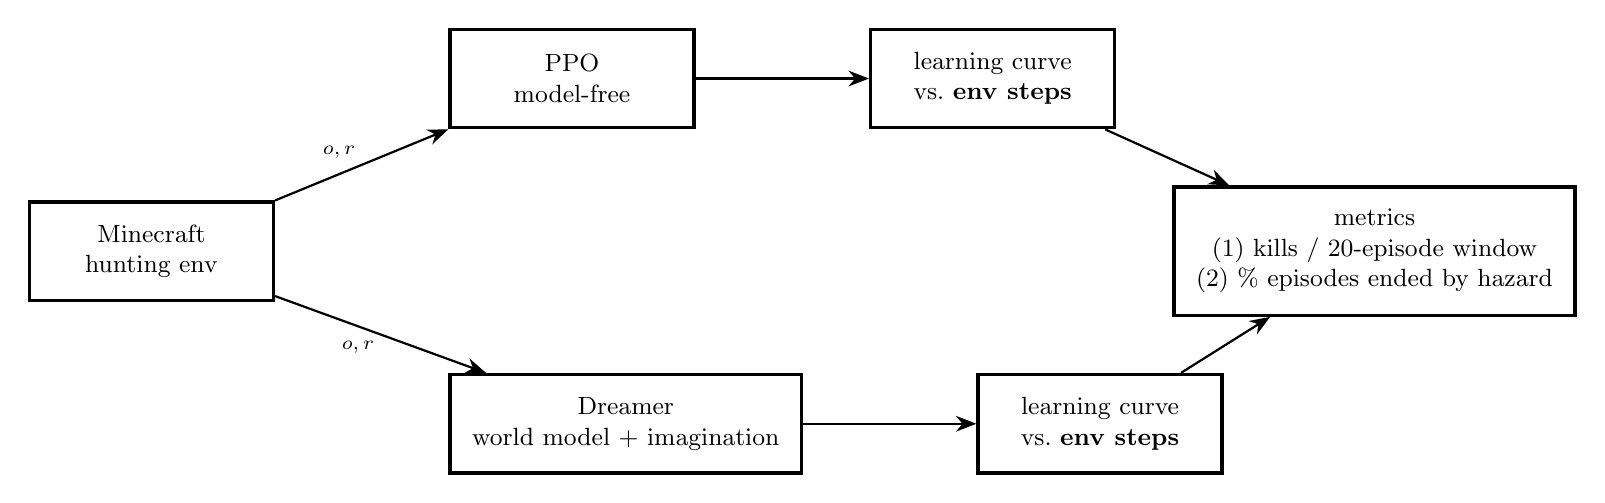
\begin{tikzpicture}[node distance=1.0cm and 1.6cm]
  \node[box] (env) {Minecraft\\hunting env};
  \node[box, above right=0.9cm and 2.2cm of env] (ppo) {PPO\\model-free};
  \node[box, below right=0.9cm and 2.2cm of env] (drm) {Dreamer\\world model $+$ imagination};
  \draw[arr] (env) -- node[lbl, above left] {$o,r$} (ppo);
  \draw[arr] (env) -- node[lbl, below left] {$o,r$} (drm);
  \node[box, right=2.2cm of ppo] (curve1) {learning curve\\vs.\ \textbf{env steps}};
  \node[box, right=2.2cm of drm] (curve2) {learning curve\\vs.\ \textbf{env steps}};
  \draw[arr] (ppo) -- (curve1);
  \draw[arr] (drm) -- (curve2);
  \node[box, right=1.6cm of $(curve1)!0.5!(curve2)$, minimum width=4.4cm] (m) {metrics\\(1) kills / 20-episode window\\(2) \% episodes ended by hazard};
  \draw[arr] (curve1) -- (m);
  \draw[arr] (curve2) -- (m);
\end{tikzpicture}
\end{document}
